\documentclass[12pt]{article}
\usepackage{amsmath,amsfonts,amssymb,amsthm,placeins}
\usepackage[pdftex]{graphicx}
\pagestyle{plain}
\title{Back Propogation Project}
\author{Daniel Haskin}
\begin{document}
\maketitle
\section{Introduction}
Backpropogation is a method by which we may train an artificial nueral network
to classify data more and more accurately. In this project, I implement the
backpropogation algorithm, and use it to find out what choices of parameters
yield the best predictive accuracy using the Iris and Vowel datasets.
\section{Methods}
\subsection{Basic Implemented Functionality}
In my implementation of the backpropogation algorithm, I implemented
the following functionality:
\begin{enumerate}
\item The neural network updates its weights incrementally
\item Ability to add arbitrarily large layers to the network using the
    \texttt{--add-layer} option
\item Random weight initialization using a standard Gaussian distribution
\item Random shuffling (randomization) of the data at the beginning of each
    training epoch.
\item Optional momentum term via the \texttt{-m} option.
\end{enumerate}
\subsection{Stopping Criteria}
 As to stopping criteria, I had a real problem. I tried all sorts of things
 with little success. At length and at the professor's advice I created
 a stopping criterion with two clauses:
 \begin{enumerate}
     \item Keep track of the best rate of accuracy so far. If this rate of
         accuracy is not improved within 50 epochs, stop.
     \item If nothing else, stop after 2500 epochs.
 \end{enumerate}
 This stopping criterion worked much better. It turns out that even looking
 for the smallest improvement within 50 epochs, the second hard-stop clause
 was never needed in my experiements. The algorithm alwasy stopped at a
 relatively appropriate time.
 \section{Choosing a Learning Rate}
 \subsection{Iris Dataset}

As per the project specifications, I looked at several different learning rates
to determine the best learning rate for the iris dataset. I tried various
learning rates using a single layer of 8 nodes. My findings are summarized in
figures \ref{fig:iris_learningrate_training} and
\ref{fig:iris_learningrate_testing}.
\begin{figure}[!ht]
    \begin{center}
        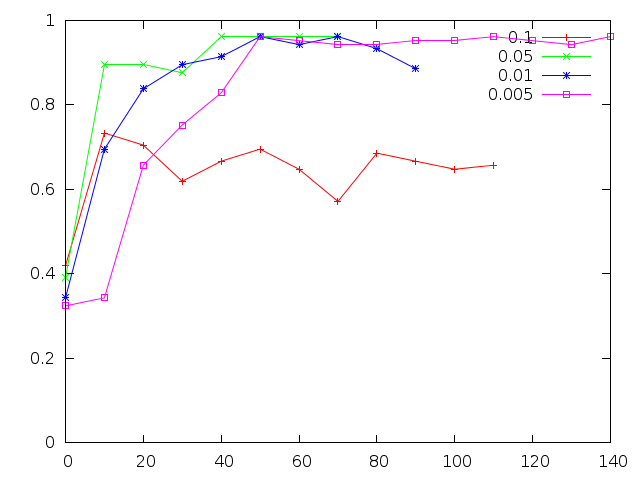
\includegraphics[width=0.65\textwidth]{iris-learningrate-training}
    \end{center}
    \caption{Training set acuracy over time with differnt learning rates using the iris dataset.}
  \label{fig:iris_learningrate_training}
\end{figure}

\begin{figure}[!ht]
    \begin{center}
        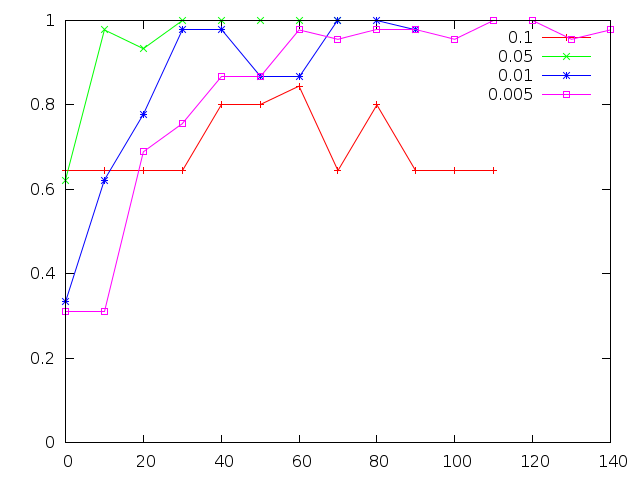
\includegraphics[width=0.65\textwidth]{iris-learningrate-testing}
    \end{center}
    \caption{Testing set accuracy over time with different learning rates using the iris dataset.}
  \label{fig:iris_learningrate_testing}
\end{figure}
It seems the best learning rate for iris is $0.05$.
\subsection{Vowel Dataset}
Doing the same experiment with the vowel dataset, using a single layer of 8
hidden nodes, we find that the best learning rate for vowel is $0.01$. See
figures \ref{fig:vowel_learningrate_training} and \ref{fig:vowel_learningrate_testing}.
\begin{figure}[!ht]
    \begin{center}
        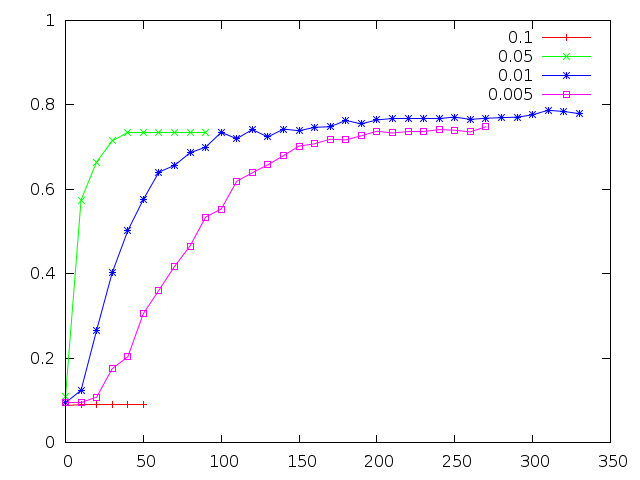
\includegraphics[width=0.65\textwidth]{vowel-learningrate-training}
    \end{center}
    \caption{Training set acuracy over time with differnt learning rates using the vowel dataset.}
  \label{fig:vowel_learningrate_training}
\end{figure}

\begin{figure}[!ht]
    \begin{center}
        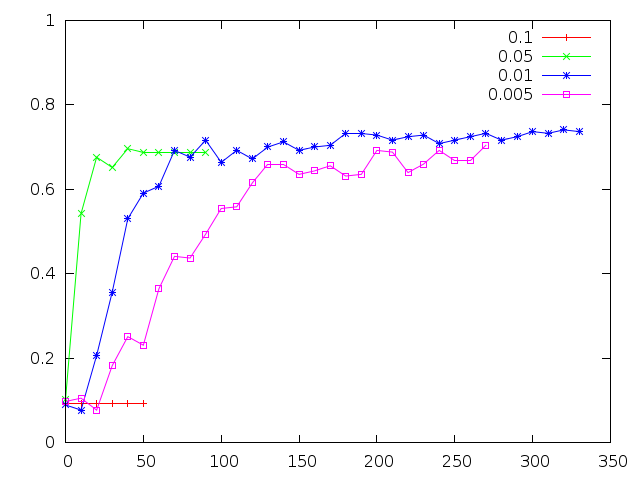
\includegraphics[width=0.65\textwidth]{vowel-learningrate-testing}
    \end{center}
    \caption{Testing set accuracy over time with different learning rates using the vowel dataset.}
  \label{fig:vowel_learningrate_testing}
\end{figure}

\section{Hidden Nodes}
\subsection{Iris Dataset}
Running various experiments with the iris dataset, using a learning rate of
$0.05$, it seems that with each node,
accuracy improves greatly. It seems that only $3$ nodes are needed to produce
optimal results. See figures
\ref{fig:iris_hiddennodes_training} and \ref{fig:iris_hiddennodes_testing}.
\begin{figure}[!ht]
    \begin{center}
        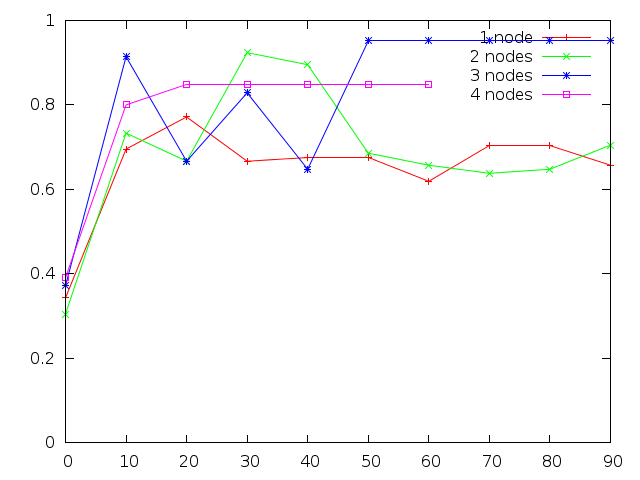
\includegraphics[width=0.65\textwidth]{iris-hiddennodes-training}
    \end{center}
    \caption{Training set acuracy over time with differnt sizes of hidden layers using the iris dataset.}
  \label{fig:iris_hiddennodes_training}
\end{figure}

\begin{figure}[!ht]
    \begin{center}
        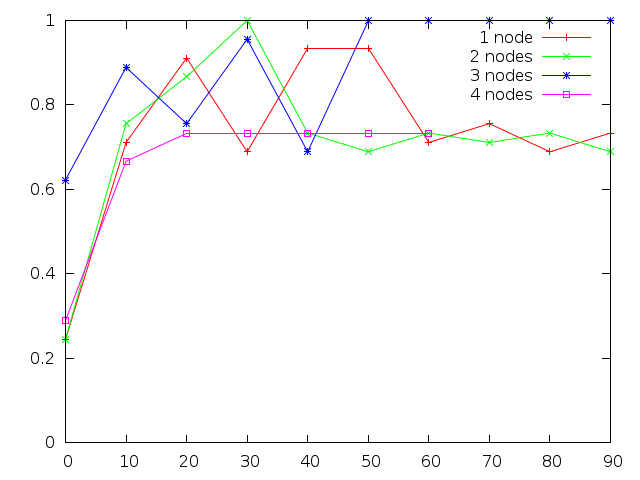
\includegraphics[width=0.65\textwidth]{iris-hiddennodes-testing}
    \end{center}
    \caption{Testing set accuracy over time with different sizes of hidden layers using the iris dataset.}
  \label{fig:iris_hiddennodes_testing}
\end{figure}
\subsection{Vowel Dataset}
Repeating the experiments with the vowel dataset, with the learning rate as
$0.01$, we find that it takes more nodes to get the same results. Incrementing
the size of the middle layer node-by-node, The accuracy started to plateu
around $10$ nodes.

\begin{figure}[!ht]
    \centering
    \begin{minipage}[b]{0.45\linewidth}
        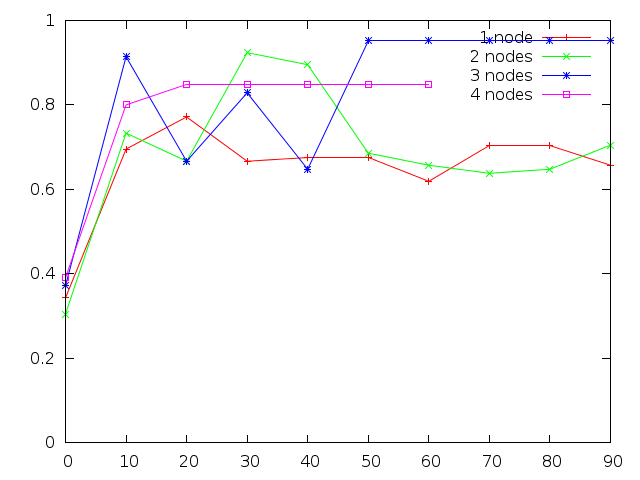
\includegraphics[width=1.0\textwidth]{iris-hiddennodes-training}
        \caption{Training set acuracy over time with differnt sizes of hidden layers using the iris dataset.}
      \label{fig:iris_hiddennodes_training}
  \end{minipage}
  \quad
    \begin{minipage}[b]{0.45\linewidth}
        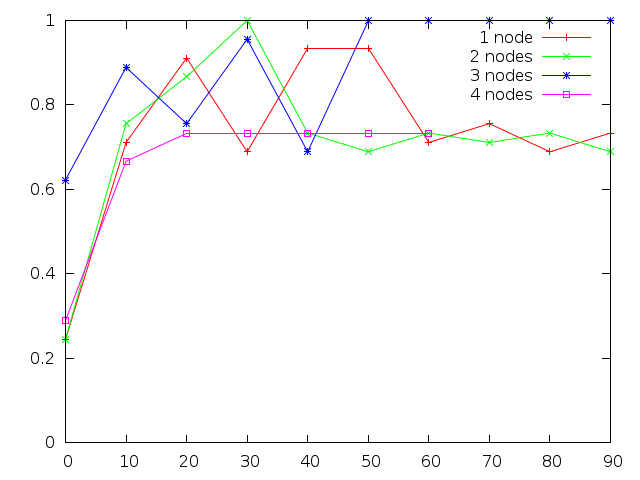
\includegraphics[width=1.0\textwidth]{iris-hiddennodes-testing}
    \caption{Testing set accuracy over time with different sizes of hidden layers using the iris dataset.}
      \label{fig:iris_hiddennodes_testing}
  \end{minipage}
\end{figure}

\begin{figure}[!ht]
    \begin{center}
    \end{center}
    \caption{Testing set accuracy over time with different sizes of hidden layers using the iris dataset.}
  \label{fig:iris_hiddennodes_testing}
\end{figure}
\end{document}
